\section{Kết quả đạt được và điểm hạn chế}
Đối với đề tài này chúng tôi đã đạt được một số kết quả nhất định.
Thứ nhất, chúng tôi đã hiện thực được không gian quản lý các dự án và các quy trình nghiệp vụ, cho phép người dùng chia sẻ không gian 
để mở rộng và cộng tác với nhiều thành viên khác trong hệ thống. Thứ hai, chúng tôi đã xây dựng được lý thuyết đánh giá chất lượng của quy
trình nghiệp vụ, cũng như lý thuyết về mức độ ưu tiên của quy trình nghiệp vụ trong một nhóm các quy trình trong Workspace. Đây là nền tảng
vững chắc để phát triển hệ thống trong giai đoạn luận văn.
\par
Tuy nhiên, đồ án tốt nghiệp vẫn còn còn một số hạn chế. Thứ nhất, hệ thống thông báo chỉ mới có hai loại thông báo cơ bản 
là thông báo về lời mời tham gia Workspace và thông báo trạng thái của yêu cầu thay đổi quyền hạn của bản thân người dùng 
trong Workspace, và chúng tôi cho rằng cần phải mở rộng hệ thống thông báo để người dùng có thể nhận được thông báo về những 
hoạt động quan trọng khác trong Workspace cũng như trong hệ thống. Thứ hai, chúng tôi chưa xử lý hết những trường hợp 
phân quyền phức tạp hơn, liên quan đến quyền hạn trong Workspace và Project. Thứ ba, tính năng thiết kế bảng khảo sát 
vẫn còn một số hạn chế, chẳng hạn như chưa linh hoạt cho phép người dùng tạo thêm các section, hay di chuyển câu hỏi 
giữa các section. Thứ tư, tính năng quản lý kết quả bảng khảo sát chưa có thêm những chức năng như xuất file báo cáo 
theo các định dạng pdf, csv, bộ lọc chi tiết kết quả thực hiện.

\section{Hướng phát triển}
Ở giai đoạn luận văn, chúng tôi sẽ tiếp tục phát triển hệ thống với những hướng phát triển sau:
\begin{itemize}
    \item Tiếp tục mở rộng hệ thống, hướng đến việc phân loại các quy trình nghiệp vụ theo từng lĩnh vực cụ thể.
    \item Nghiên cứu, phát triển các tính năng liên quan đến việc đề xuất các mẫu quy trình thuộc lĩnh vực liên quan đến quy trình hiện tại hoặc nhu cầu của người dùng.
    \item Mở rộng thêm các tính năng đóng góp, cho phép người dùng đóng góp những quy trình, góp phần xây dựng cộng đồng phát triển quy trình nghiệp vụ.
    \item Tổ chức Workspace, Project chặt chẽ hơn, phát triển thêm những tính năng quản trị.
    \item Nghiên cứu, mở rộng thêm các hướng tiếp cận để đánh giá quy trình nghiệp vụ khách quan và chính xác hơn.
\end{itemize}

% \section{Kế hoạch làm việc dự kiến cho giai đoạn luận văn}
% Dựa vào những hướng phát triển đã đề ra, chúng tôi vạch ra kế hoạch làm việc dự kiến cho giai đoạn luận văn như sau:
% \begin{figure}[H]
%     \centering
%     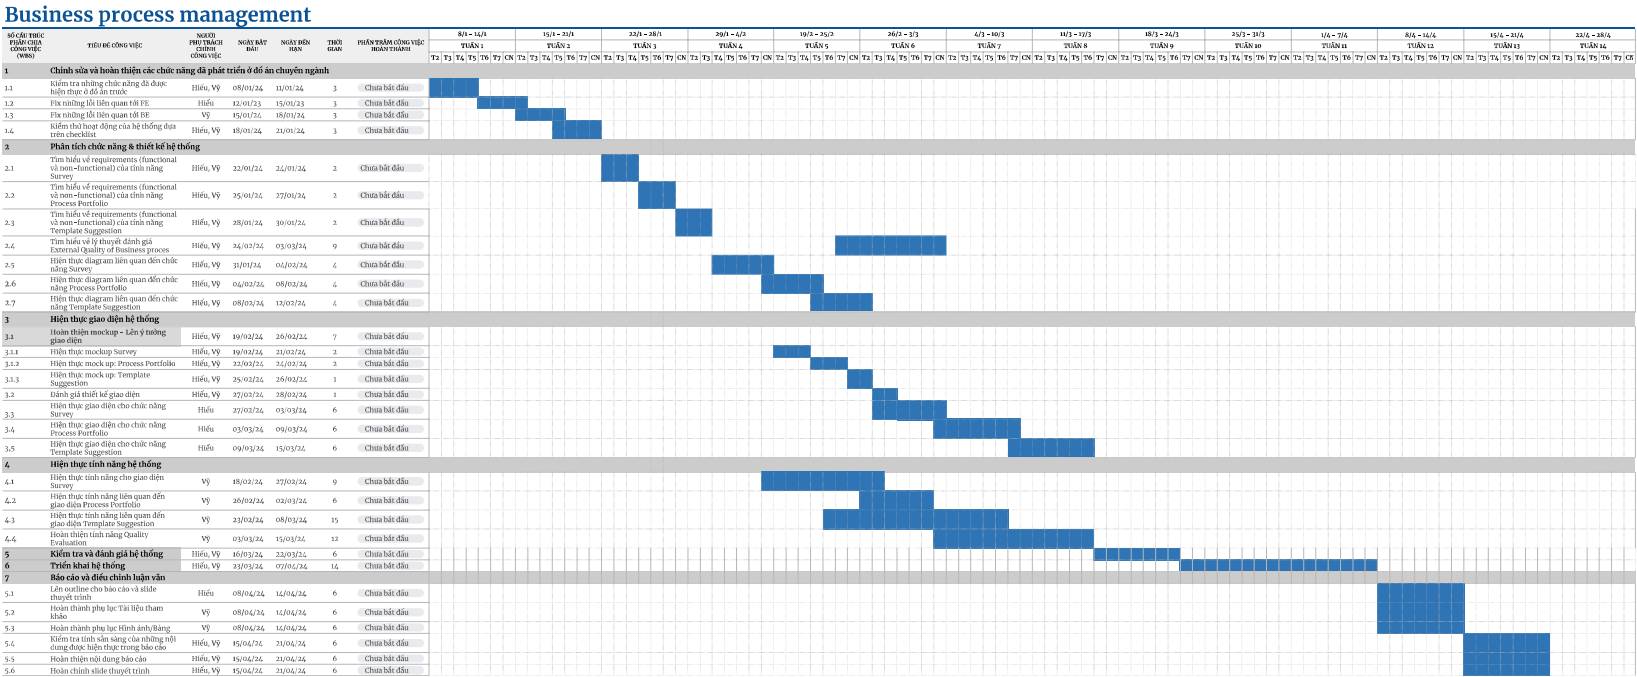
\includegraphics[width=\linewidth]{Content/Kết luận/images/graduteschedule.png}
%     \vspace{0.5cm}
%     \caption{Biểu đồ Gantt cho kế hoạch làm việc dự kiến cho giai đoạn luận văn}
%     \label{fig:Biểu đồ Gantt cho kế hoạch làm việc dự kiến cho giai đoạn luận văn}
% \end{figure}
% Mô tả chi tiết cho kế hoạch làm việc ở giai đoạn luận văn sẽ được trình bày ở bảng bên dưới.

% \newpage
% \begin{table}[H]
%     \def\arraystretch{2}
%     \resizebox{\textwidth}{!}{
%     \begin{tabular}{|p{11cm}|p{1.75cm}|p{1.5cm}|p{1.5cm}|}
%       \hline
%       \textbf{Chi tiết công việc} &
%         \multicolumn{1}{l|}{\textbf{Phân công}} &
%         \textbf{Ngày bắt đầu} &
%         \textbf{Ngày kết thúc} \\ \hline
%       Kiểm tra những chức năng đã được hiện thực ở đồ án trước        & Hiếu, Vỹ & 08/01/24 & 11/01/24 \\ \hline
%       Fix những lỗi liên quan tới FE                                  & Hiếu     & 12/01/23 & 15/01/23 \\ \hline
%       Fix những lỗi liên quan tới BE                                  & Vỹ       & 15/01/24 & 18/01/24 \\ \hline
%       Kiểm thử hoạt động của hệ thống dựa trên checklist              & Hiếu, Vỹ & 18/01/24 & 21/01/24 \\ \hline
%       Tìm hiểu về requirements (functional và non-functional) của tính năng Survey &
%         Hiếu, Vỹ &
%         22/01/24 &
%         24/01/24 \\ \hline
%       Tìm hiểu về requirements (functional và non-functional) của tính năng Process Portfolio &
%         Hiếu, Vỹ &
%         25/01/24 &
%         27/01/24 \\ \hline
%       Tìm hiểu về requirements (functional và non-functional) của tính năng Template Suggestion &
%         Hiếu, Vỹ &
%         28/01/24 &
%         30/01/24 \\ \hline
%       Tìm hiểu về lý thuyết đánh giá External Quality of Business process &
%         Hiếu, Vỹ &
%         24/02/24 &
%         03/03/24 \\ \hline
%       Hiện thực diagram liên quan đến chức năng Survey                & Hiếu, Vỹ & 31/01/24 & 04/02/24 \\ \hline
%       Hiện thực diagram liên quan đến chức năng Process Portfolio &
%         Hiếu, Vỹ &
%         04/02/24 &
%         08/02/24 \\ \hline
%       Hiện thực diagram liên quan đến chức năng Template Suggestion &
%         Hiếu, Vỹ &
%         08/02/24 &
%         12/02/24 \\ \hline
%       Hoàn thiện mockup - Lên ý tưởng giao diện                       & Hiếu, Vỹ & 19/02/24 & 26/02/24 \\ \hline
%       Hiện thực mockup Survey                                         & Hiếu, Vỹ & 19/02/24 & 21/02/24 \\ \hline
%       Hiện thực mock up: Process Portfolio                            & Hiếu, Vỹ & 22/02/24 & 24/02/24 \\ \hline
%       Hiện thực mock up: Template Suggestion                          & Hiếu, Vỹ & 25/02/24 & 26/02/24 \\ \hline
%       Đánh giá thiết kế giao diện                                     & Hiếu, Vỹ & 27/02/24 & 28/02/24 \\ \hline
%       Hiện thực giao diện cho chức năng Survey                        & Hiếu     & 27/02/24 & 03/03/24 \\ \hline
%       Hiện thực giao diện cho chức năng Process Portfolio             & Hiếu     & 03/03/24 & 09/03/24 \\ \hline
%       Hiện thực giao diện cho chức năng Template Suggestion           & Hiếu     & 09/03/24 & 15/03/24 \\ \hline
%       Hiện thực tính năng cho giao diện Survey                        & Vỹ       & 18/02/24 & 27/02/24 \\ \hline
%       Hiện thực tính năng liên quan đến giao diện Process Portfolio   & Vỹ       & 26/02/24 & 02/03/24 \\ \hline
%       Hiện thực tính năng liên quan đến giao diện Template Suggestion & Vỹ       & 23/02/24 & 08/03/24 \\ \hline
%       Hoàn thiện tính năng Quality Evaluation                         & Vỹ       & 03/03/24 & 15/03/24 \\ \hline
%     \end{tabular}}
%     \vspace{0.5cm}
%     \caption{Bảng kế hoạch công việc chi tiết cho giai đoạn luận văn}
% \end{table}

% \begin{table}[H]
%     \def\arraystretch{2}
%     \resizebox{\textwidth}{!}{
%     \begin{tabular}{|p{11cm}|p{1.75cm}|p{1.5cm}|p{1.5cm}|}
%       \hline
%       \textbf{Chi tiết công việc} &
%         \multicolumn{1}{l|}{\textbf{Phân công}} &
%         \textbf{Ngày bắt đầu} &
%         \textbf{Ngày kết thúc} \\ \hline
%       Kiểm tra và đánh giá hệ thống                                   & Hiếu, Vỹ & 16/03/24 & 22/03/24 \\ \hline
%       Triển khai hệ thống                                             & Hiếu, Vỹ & 23/03/24 & 07/04/24 \\ \hline
%       Lên outline cho báo cáo và slide thuyết trình                   & Hiếu     & 08/04/24 & 14/04/24 \\ \hline
%       Hoàn thành phụ lục Tài liệu tham khảo                           & Vỹ       & 08/04/24 & 14/04/24 \\ \hline
%       Hoàn thành phụ lục Hình ảnh/Bảng                                & Vỹ       & 08/04/24 & 14/04/24 \\ \hline
%       Kiểm tra tính sẵn sàng của những nội dung được hiện thực trong báo cáo &
%         Hiếu, Vỹ &
%         15/04/24 &
%         21/04/24 \\ \hline
%       Hoàn thiện nội dung báo cáo                                     & Hiếu, Vỹ & 15/04/24 & 21/04/24 \\ \hline
%       Hoàn chỉnh slide thuyết trình                                   & Hiếu, Vỹ & 15/04/24 & 21/04/24 \\ \hline
%     \end{tabular}}
%     \vspace{0.5cm}
%     \caption{Bảng kế hoạch công việc chi tiết cho giai đoạn luận văn - tiếp theo}
% \end{table}